\chapter{Návrh systému}
% tady popsat, jak jsme systém navrhovali.
Návrh monitorovacího systému vychází z~analýzy provozních požadavků na nepřetržité zpracování obrazového toku v~reálném čase přímo v~místě instalace kamery. Při koncepčním návrhu byla zvolena metodika dekompozice systému do pěti funkčně nezávislých vrstev, které jsou vzájemně propojeny asynchronními komunikačními kanály. Tato kapitola postupně definuje funkční a nefunkční požadavky, představuje celkovou distribuovanou architekturu a zdůvodňuje volbu hardwarových prvků v~čele s~jednodeskovým počítačem Raspberry Pi~5 a akcelerátorem Hailo-8. Dále je detailně rozpracován objektový návrh aplikace pomocí diagramu tříd \acs{UML}, logika prostorové filtrace vozidel v~polygonální zóně \acs{ROI}, mechanismus asynchronního přenosu zpráv protokolem \acs{MQTT} a návrh relačního datového modelu v~databázi PostgreSQL včetně strategie indexování a následné analytické vizualizace.

\section{Požadavky na systém}
Navrhovaný systém je určen pro automatizovanou analýzu silniční dopravy 
pomocí metod počítačového vidění. Cílem je detekce a sledování vozidel 
v~reálném čase a následná extrakce statistických údajů o~jejich průjezdech.

Mezi hlavní funkční požadavky patří:

\begin{itemize}
    \item detekce vozidel v~obrazové sekvenci,
    \item klasifikace detekovaných vozidel do kategorií,
    \item sledování klasifikovaných objektů napříč jednotlivými snímky,
    \item identifikace průjezdu klasifikovaných objektů definovanou oblastí zájmu (\acs{ROI}),
    \item ukládání detekčních událostí do databáze,
    \item vizualizace agregovaných statistik.
\end{itemize}

Systém musí být schopen provozu v~reálném čase na vestavěném zařízení s~omezenými výpočetními prostředky. Z~tohoto důvodu je navržena architektura založená na principu \textit{edge computing}, kdy je inference neuronové sítě prováděna přímo na zařízení v~místě sběru dat~\cite{akira_edge_cloud}.

\section{Celková architektura a tok dat}

%Architektura systému je navržena jako vícevrstvá a modulární. 
%Jednotlivé komponenty jsou odděleny podle své funkce, což umožňuje lepší škálovatelnost, robustnost a údržbu systému.


Architektura systému je navržena jako vícevrstvá, distribuovaná a modulární. Jednotlivé komponenty jsou odděleny podle své funkce a komunikují spolu asynchronně prostřednictvím lehkého zprávového protokolu MQTT~\cite{mqtt_oasis_2019}. Toto rozdělení umožňuje lepší škálovatelnost, robustnost a minimalizaci vzájemné závislosti komponent, což plně odpovídá moderním architekturám dopravních monitorovacích systémů založených na počítačovém vidění~\cite{zhou_traffic_survey_2024}.

% upravit návrh komunikace v šipky na obě dvě strany mezi moduly
\begin{figure}[H]
    \centering
    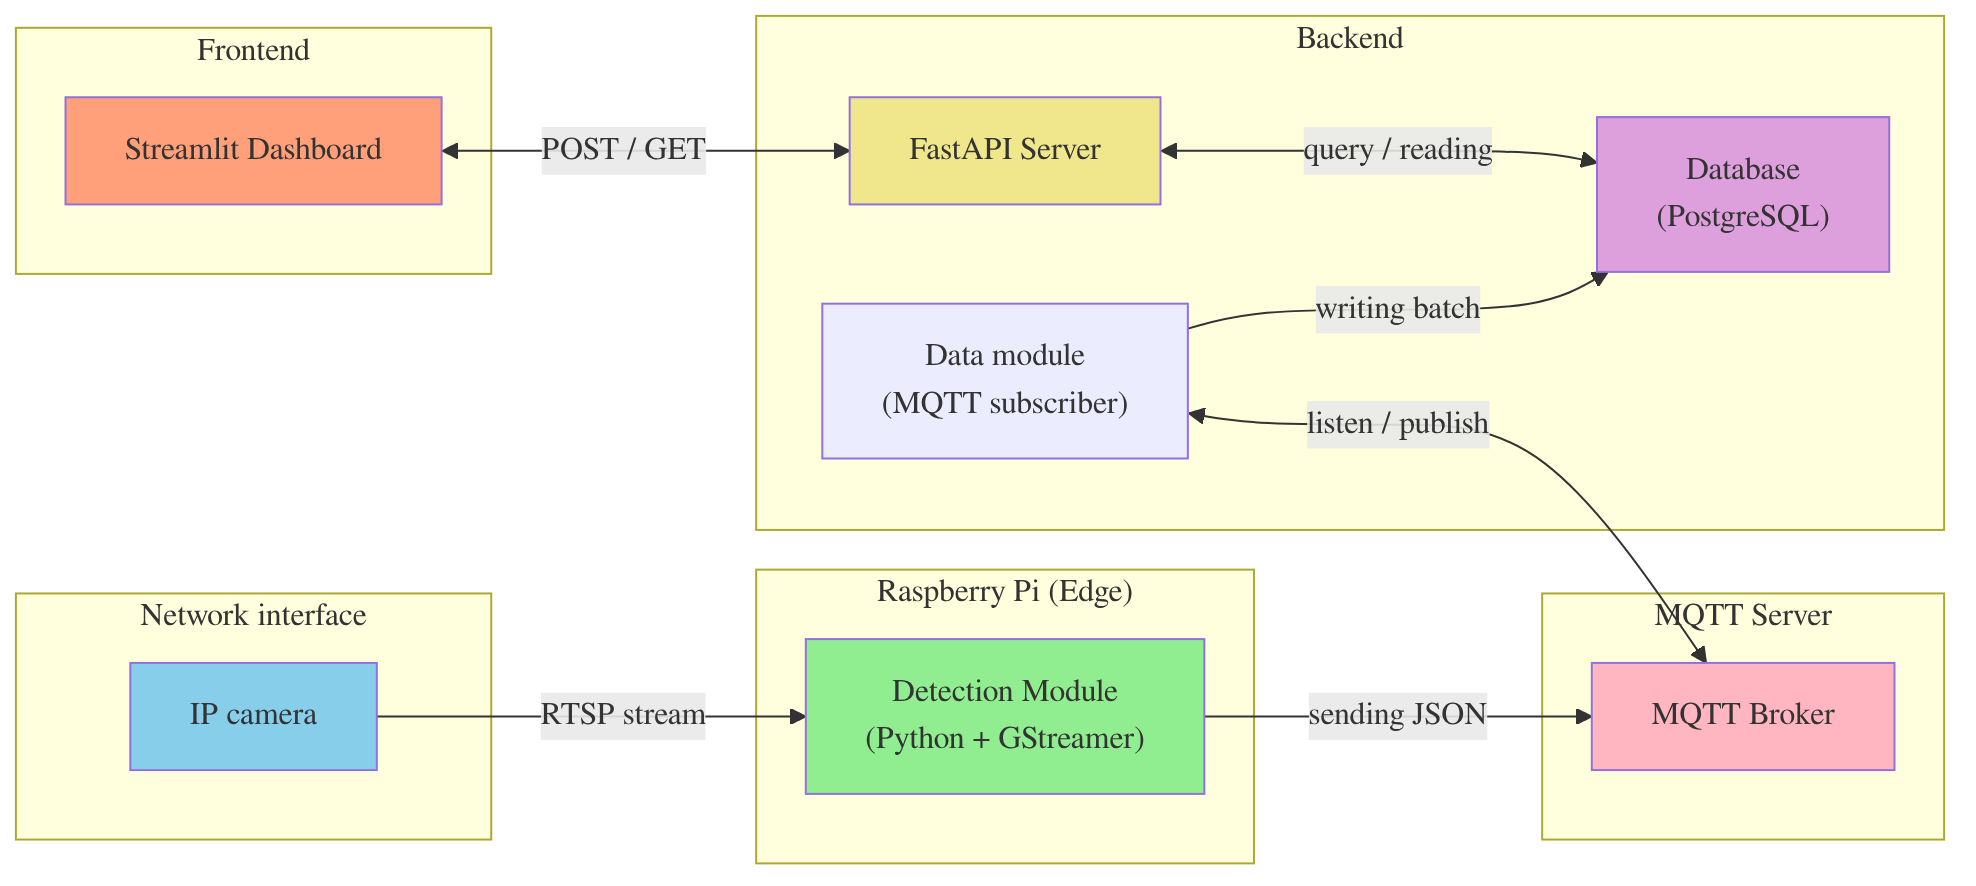
\includegraphics[width=\textwidth]{images/architecture.png}
    \caption{Navržená architektura systému pro analýzu dopravy}
    \label{fig:architecture}
\end{figure}

Na obrázku~\ref{fig:architecture} je znázorněna celková topologie navrženého řešení a~směr komunikace mezi komponentami. Systém je rozdělen do pěti funkčních vrstev, kterými postupně prochází tok dat:

\begin{enumerate}
    \item \textbf{Vrstva akvizice a~výstupu obrazu (Síťová vrstva):} Koncová \acs{IP} kamera poskytuje kontinuální video stream přenášený po lokální síti pomocí protokolu \acs{RTSP}. Do této vrstvy může okrajový modul volitelně vracet také zpracovaný obrazový stream s~vykreslenými detekcemi (přes lokální \acs{RTSP} server) nebo jej ukládat do video souboru MP4.
    \item \textbf{Vrstva zpracování videa (Edge vrstva):} Obrazová data jsou přijata na okrajovém zařízení v~řetězci GStreamer, předzpracována a~předána detekčnímu modelu \acs{YOLO}~\cite{redmon_yolo_2016} na akcelerátoru Hailo-8. Následný sledovací algoritmus (na principu \acs{SORT}~\cite{SORT_original_2016}) přiřazuje objektům unikátní identifikátory a~vyhodnocuje jejich průchod definovanou oblastí zájmu (\acs{ROI})~\cite{mdpi_roi_tracking_2022}. Pro testovací a~ladicí účely dokáže tento modul zpracovaný obraz s~vykreslenými detekcemi souběžně vysílat jako výstupní \acs{RTSP} stream nebo ukládat do souboru MP4.
    \item \textbf{Komunikační vrstva (\acs{MQTT} Server):} Vygenerované strukturované události o~průjezdech jsou ve formátu \acs{JSON} jednosměrně odesílány (\textit{sending}) do centrálního \acs{MQTT} brokeru~\cite{mqtt_oasis_2019}.
    \item \textbf{Datová a~backendová vrstva:} Datový modul (\acs{MQTT} subscriber) udržuje obousměrné spojení s~brokerem (\textit{listen / publish} pro odebírání zpráv a~potvrzování stavů) a~přijaté události dávkově zapisuje (\textit{writing}) do relační databáze PostgreSQL. Součástí backendu je aplikační server FastAPI, který s~databází komunikuje obousměrně (\textit{query / reading}) – odesílá analytické \acs{SQL} dotazy a~přijímá výsledné datové sady.
    \item \textbf{Aplikační a~vizualizační vrstva (Frontend):} Webový dashboard ve frameworku Streamlit komunikuje s~FastAPI serverem obousměrně přes protokol \acs{HTTP} (\textit{POST / GET}) – pomocí požadavků \texttt{GET} načítá agregované dopravní statistiky pro grafy a~pomocí požadavků \texttt{POST} umožňuje administrátorovi vzdáleně spouštět či zastavovat detekční pipeline a~databázové služby.
\end{enumerate}

Oddělení jednotlivých kroků do samostatných vrstev umožňuje vysokou modularitu systému a minimalizaci vzájemné závislosti komponent.

\section{Výběr hardwaru}
Pro zajištění spolehlivého chodu celého řešení je hardwarová část fyzicky rozdělena na prvek pro sběr obrazových dat a výpočetní uzel pro jejich zpracování.

\textbf{Kamerový systém:} Pro dosažení dostatečné kvality detekce je využita IP kamera značky Hikvision, která umožňuje síťový přenos video streamu prostřednictvím protokolů \acs{RTSP} nebo \acs{HTTP}. Použití IP kamery dovoluje flexibilní umístění zařízení mimo samotný výpočetní uzel a současně poskytuje vyšší odolnost vůči povětrnostním podmínkám v~porovnání s~běžnými kamerovými moduly pro vestavěná zařízení. %Kamera poskytuje obraz ve vysokém rozlišení, což je klíčové pro přesnou detekci vozidel zejména ve větší vzdálenosti od kamery.

\textbf{Zpracovatelská jednotka:} Jako výpočetní platforma na hraně sítě (edge zařízení), která přijímá datový tok z~lokální sítě, je navrženo zařízení Raspberry Pi 5. Tato platforma představuje vhodný kompromis mezi výkonem, spotřebou a pořizovací cenou~\cite{raspberrypi_docs_2024}. Pro zajištění real-time inference neuronové sítě je doplněna o~dedikovaný AI akcelerátor Hailo-8 kompatibilní s~touto platformou~\cite{raspberrypi_ai_kit}. Tento přístup umožňuje efektivní zpracování obrazu přímo na místě bez nutnosti využití cloudových služeb.

\textbf{Referenční výpočetní stanice (\acs{GPU}):} Pro účely kompilace modelů (která je paměťově i~výpočetně náročná) a~pro realizaci referenčního srovnávacího měření s~nekvantizovaným modelem \acs{YOLO} v~plné přesnosti (FP32/FP16) byl zvolen přenosný počítač Acer Nitro~V~15 (ANV15-51) vybavený dedikovanou grafickou kartou \textbf{NVIDIA GeForce RTX~2050} (architektura Ampere, 2\,048~CUDA jader, 4~GB paměti GDDR6). Tato platforma slouží v~experimentální části práce jako referenční srovnávací základna vůči nízkoenergetickému okrajovému uzlu s~akcelerátorem Hailo-8.

\section{Návrh softwarových modulů}
%Softwarová architektura je navržena jako distribuovaná a asynchronní. Jednotlivé komponenty komunikují prostřednictvím lehkého zprávového protokolu MQTT \cite{mqtt_oasis_2019}.

\subsection{Objektový návrh aplikace (UML)}
Pro zajištění modularity, snadné testovatelnosti a budoucí rozšiřitelnosti byl softwarový kód systému navržen s~využitím objektově orientovaného programování (OOP). Jednotlivé funkční celky od zpracování videa přes mezivrstvu pro přenos zpráv až po databázové operace a aplikační rozhraní, jsou zapouzdřeny do samostatných tříd a modulů (viz obrázek~\ref{fig:class_diagram}). Tento přístup umožňuje provozovat detekční část zcela autonomně z~příkazové řádky, nebo ji dynamicky řídit prostřednictvím webového rozhraní.

\begin{figure}[H]
    \centering
    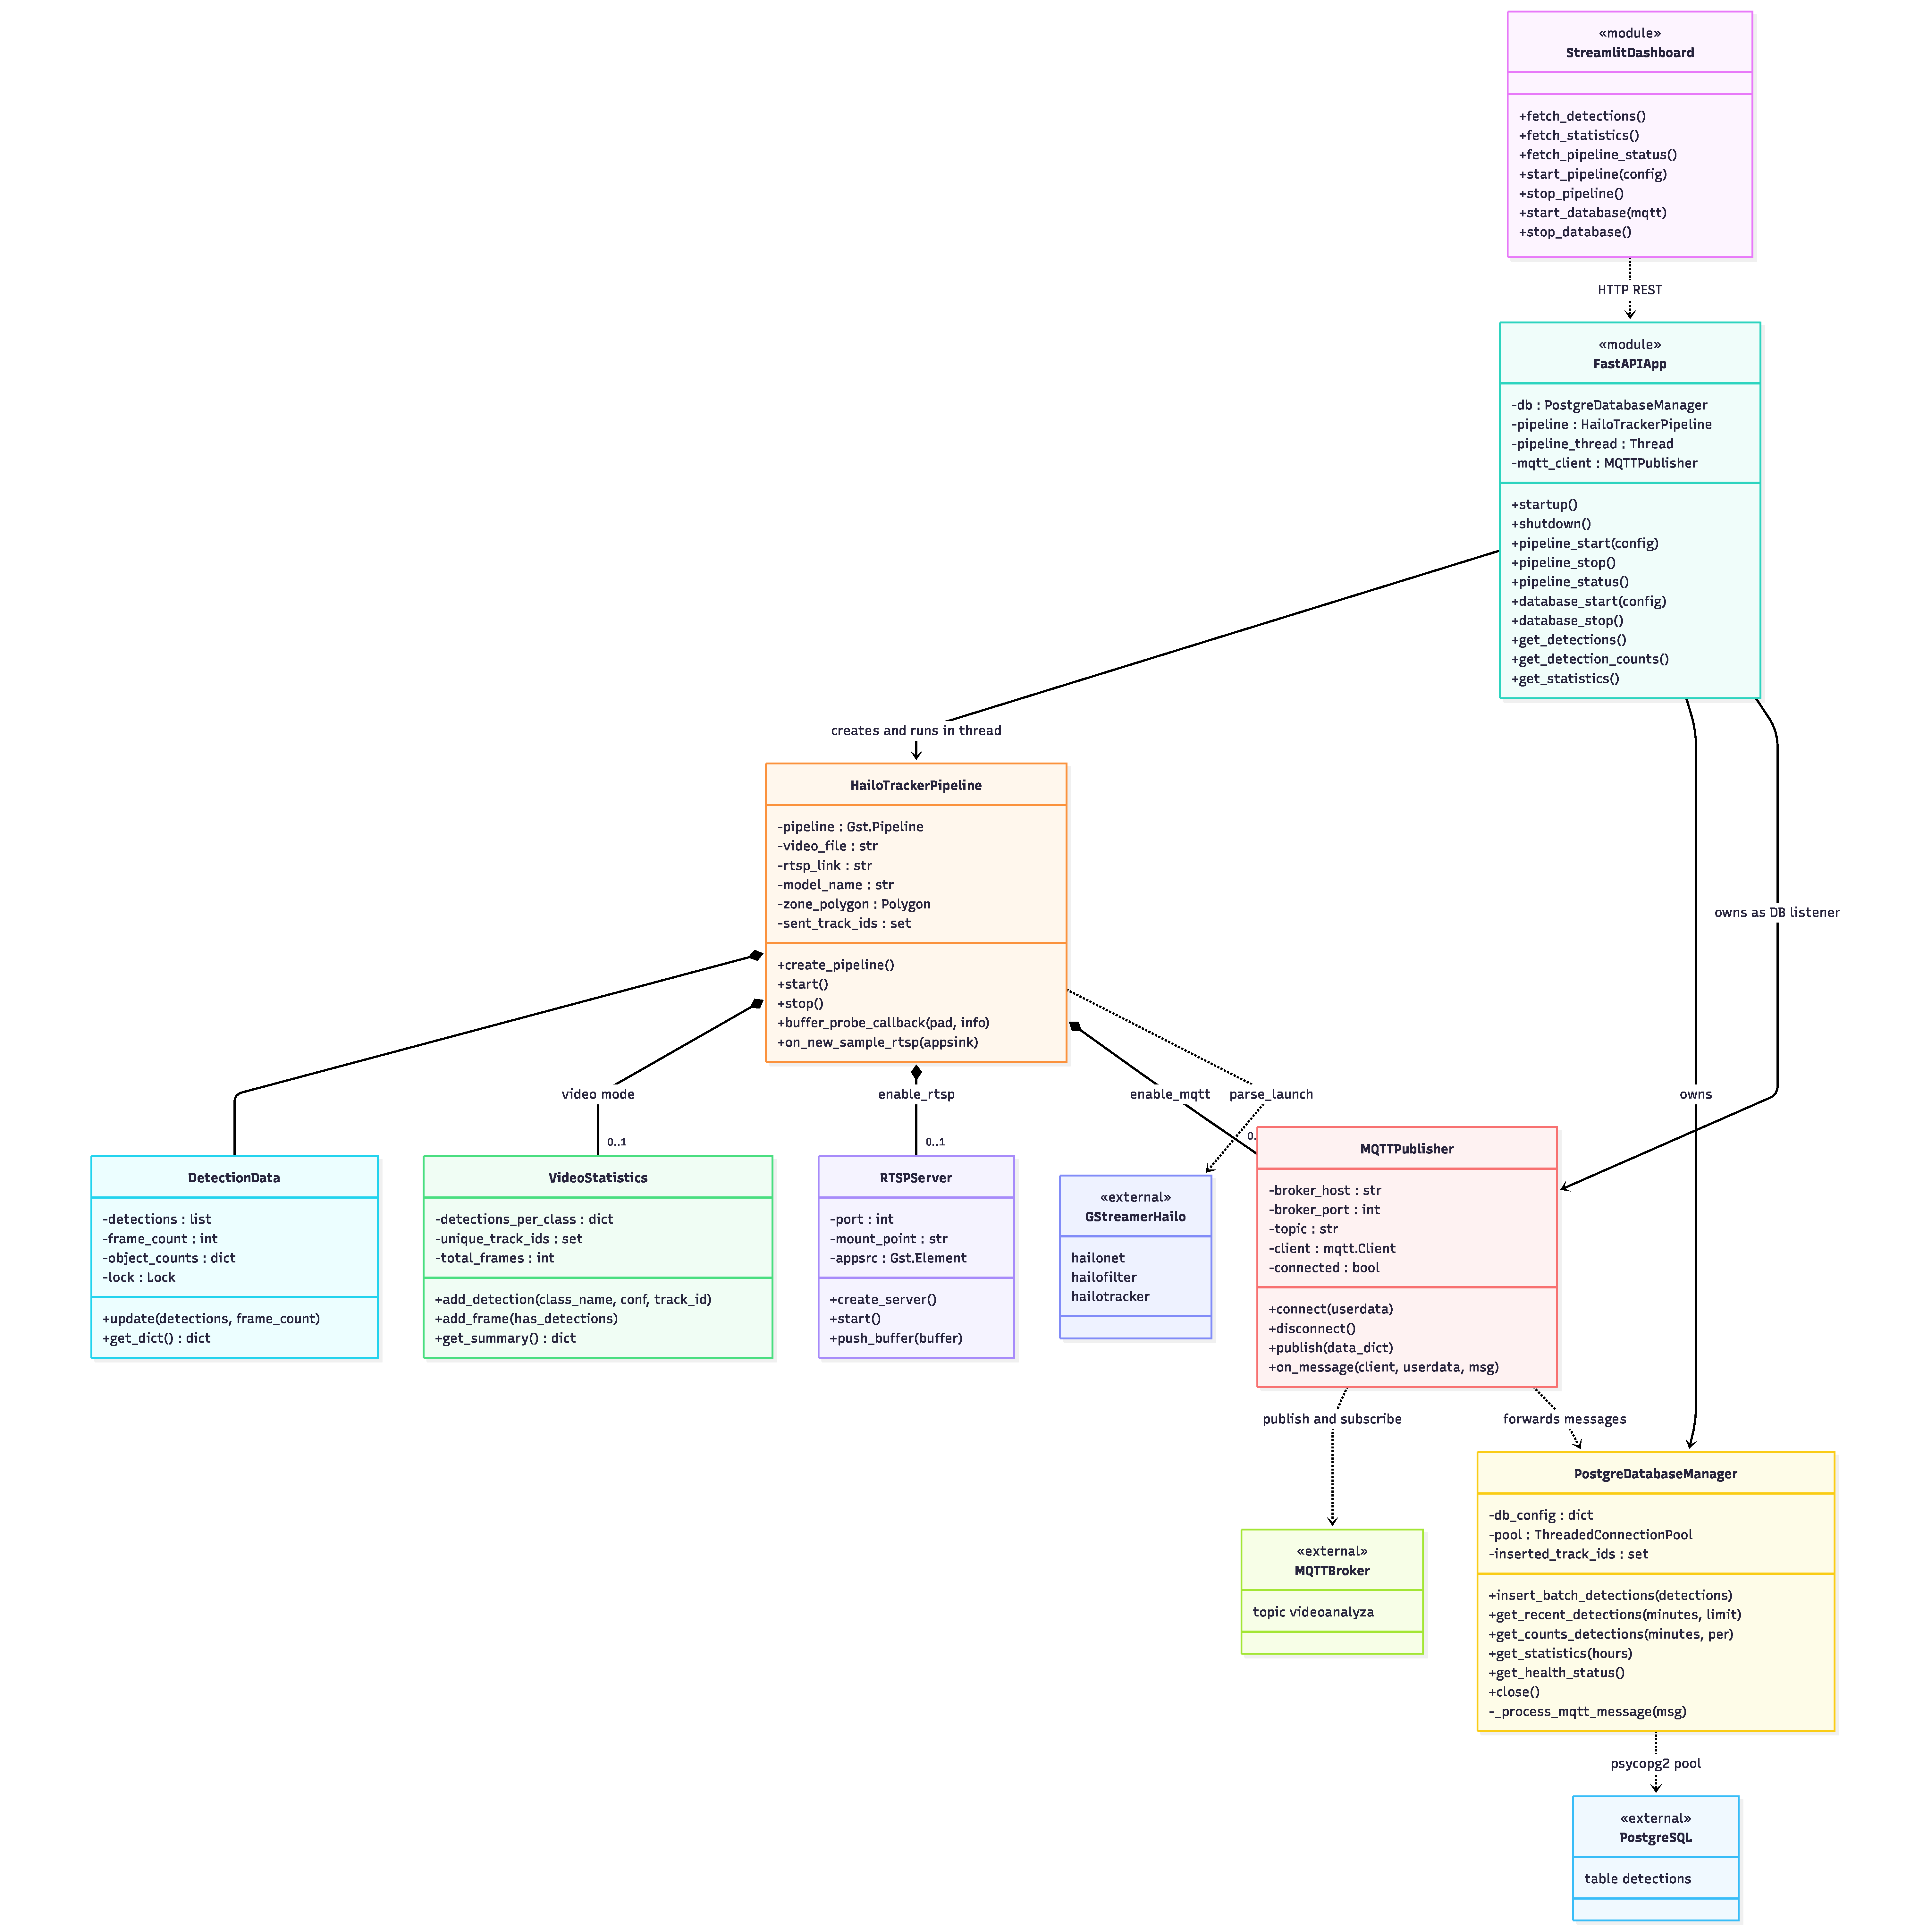
\includegraphics[
        page=1,    
    width=1\textwidth
    ]{images/System_UML.pdf}
    \caption{UML diagram tříd navrženého dopravního monitorovacího systému.}
    \label{fig:class_diagram}
\end{figure}

Struktura softwarové aplikace se skládá z~následujících klíčových tříd a modulů:
\begin{itemize}
    \item \textbf{\texttt{HailoTrackerPipeline}} – Ústřední třída detekčního modulu na hraně sítě. Zapouzdřuje sestavení a řízení multimediálního řetězce (\texttt{Gst.Pipeline}), komunikaci s~akcelerátorem Hailo-8 a registraci zpětného volání (\texttt{buffer\_probe\_callback}). Současně udržuje geometrickou definici oblasti zájmu (\texttt{zone\_polygon}) a množinu již odeslaných identifikátorů (\texttt{sent\_track\_ids}) pro eliminaci duplicit.
    \item \textbf{\texttt{DetectionData}} – Datová struktura zajišťující vláknově bezpečné (\textit{thread-safe}) uchovávání aktuálních výsledků detekce a počtů objektů pomocí synchronizačního zámku (\texttt{Lock}). Poskytuje metody pro serializaci dat do slovníku a generování překryvného textu do obrazu.
    \item \textbf{\texttt{VideoStatistics}} a \textbf{\texttt{RTSPServer}} – Volitelné (kompozičně vázané) pomocné třídy. \texttt{VideoStatistics} slouží k~agregaci souhrnných metrik při zpracování video souborů, zatímco \texttt{RTSPServer} umožňuje prostřednictvím prvku \texttt{appsrc} přeposílat zpracovaný video stream s~vykreslenými detekcemi dále do sítě.
    \item \textbf{\texttt{MQTTPublisher}} – Univerzální komunikační třída zapouzdřující klienta protokolu MQTT. V~architektuře plní dvojí roli: na straně detekční pipeline zajišťuje publikaci dat (\texttt{publish}) do tématu \texttt{videoanalyza}, zatímco na straně serveru funguje jako odběratel (\textit{listener}), který přijaté zprávy předává metodě \texttt{on\_message} ke zpracování do databáze.
    \item \textbf{\texttt{PostgreDatabaseManager}} – Třída zodpovědná za perzistenci a čtení dat z~relační databáze PostgreSQL. Využívá fond spojení (\texttt{ThreadedConnectionPool}) z~knihovny \texttt{psycopg2}, zpracovává příchozí MQTT zprávy, provádí dávkové vkládání záznamů (\texttt{insert\_batch\_detections}) a poskytuje agregační metody pro analytické dotazy.
    \item \textbf{\texttt{FastAPIApp}} a \textbf{\texttt{StreamlitDashboard}} – Aplikační a prezentační moduly. Modul \texttt{FastAPIApp} poskytuje REST API rozhraní pro čtení statistik z~databáze a zároveň umožňuje vzdáleně spouštět a zastavovat detekční pipeline v~samostatném vlákně (\texttt{Thread}). Modul \texttt{StreamlitDashboard} s~tímto rozhraním komunikuje přes protokol HTTP a zajišťuje interaktivní vizualizaci dat pro koncového uživatele.
\end{itemize}

\subsection{Detekční modul a logika počítání (ROI)}
Detekční modul je založen na konvoluční neuronové síti typu \acs{YOLO}, která umožňuje rychlou lokalizaci a klasifikaci objektů v~obraze~\cite{redmon_yolo_2016}. Pro následné sledování těchto objektů napříč snímky je navržen algoritmus na principu \acs{SORT}~\cite{SORT_original_2016} (v~rámci hardwarově optimalizovaného modulu \texttt{hailotracker}), případně \acs{DeepSORT}~\cite{wojke_deepsort_2017} či ByteTrack. Každému sledovanému objektu je tak přiřazen unikátní identifikátor (\acs{ID}), jenž je udržován po celou dobu jeho výskytu ve scéně.

\textbf{Logika detekční zóny (ROI):}
Pro účely filtrace a počítání relevantních vozidel je v~obraze definována virtuální oblast zájmu (\acs{ROI}) ve tvaru obecného polygonu~\cite{mdpi_roi_tracking_2022}. Polygonální reprezentace (implementovaná pomocí geometrické knihovny Shapely) umožňuje přesně vymezit sledovaný jízdní pruh na okružní křižovatce a odfiltrovat nežádoucí detekce mimo komunikaci. Započítání vozidla proběhne v~okamžiku, kdy se geometrický střed jeho ohraničujícího rámečku (\textit{bounding box}) ocitne uvnitř definovaného polygonu. Aby nedocházelo k~vícenásobnému započítání téhož vozidla v~po sobě jdoucích snímcích, systém udržuje v~paměti množinu již zpracovaných identifikátorů \texttt{track\_id} a každé unikátní vozidlo odešle ke zpracování pouze jednou.

% rozebrat to co mám popsané v závěru (posílání, zpracování dat)

\subsection{Zpracování datového toku a asynchronního přenosu}
Aby okrajové zařízení zvládalo zpracovávat obrazový tok v~reálném čase bez ztráty snímků, je vnitřní zpracování dat navrženo jako striktně oddělené (decoupled) na úrovni multimediálního zpracování i síťové komunikace:

\begin{enumerate}
    \item \textbf{Zřetězené zpracování obrazu (GStreamer pipeline):} Dekódování síťového \acs{RTSP} streamu, změna rozlišení na $640 \times 640$~pixelů, samotná inference na čipu Hailo-8 (ze zkompilovaného binárního souboru \acs{HEF}) a přiřazování sledovacích identifikátorů jsou navrženy jako souvislý datovod v~nativním C/C++ frameworku GStreamer. Řídicí vrstva v~jazyce Python do obrazových matic přímo nezasahuje, ale pouze odebírá vygenerovaná textová metadata o~detekcích prostřednictvím asynchronního zpětného volání (\textit{buffer probe}).
    \item \textbf{Asynchronní přenos metadat (\acs{MQTT} návrh):} Přímý synchronní zápis do vzdálené databáze z~vlákna zpracovávajícího video by v~případě síťové odezvy blokoval výpočetní pipeline. Proto je přenos dat navržen na bázi modelu \textit{Publish/Subscribe} pomocí protokolu \acs{MQTT}~\cite{mqtt_oasis_2019}. Jakmile vozidlo projede polygonální zónou \acs{ROI}, detekční modul sestaví lehkou datovou zprávu ve formátu \acs{JSON} (obsahující identifikátor a název třídy, míru spolehlivosti \textit{confidence}, souřadnice rámečku \texttt{bbox}, sledovací \texttt{track\_id} a časové razítko \texttt{timestamp}) a neblokujícím způsobem ji publikuje na \acs{MQTT} broker do tématu \texttt{/videoanalyza}.
    \item \textbf{Dávková perzistence a obsluha dotazů (\acs{REST} \acs{API}):} Na straně serveru odebírá zprávy z~\acs{MQTT} brokeru nezávislá služba (subscriber). Pro minimalizaci režie databázových transakcí při hustém provozu je navrženo využití fondu spojení (\textit{connection pooling}) a dávkového vkládání záznamů (\textit{batch insert}). Nad databází stojí backendový server ve frameworku FastAPI, který prostřednictvím \acs{REST} \acs{API} endpointů poskytuje předagregovaná statistická data prezentační vrstvě (Streamlit dashboardu) a současně umožňuje vzdálené řízení stavu detekční pipeline.
\end{enumerate}

\subsection{Ukládání dat, databázové schéma a vizualizace}
Strukturované detekční události jsou ukládány do relační databáze PostgreSQL, která umožňuje spolehlivé uchování dat a jejich následné statistické vyhodnocení~\cite{psycopg_docs_2025}. Pro účely trvalé evidence byla navržena primární tabulka \texttt{detections}, jejíž struktura je znázorněna na obrázku~\ref{fig:erd}. Každý zaznamenaný průjezd unikátního vozidla definovanou zónou \acs{ROI} vygeneruje právě jeden záznam.

\subsubsection{Datový model}
Datový model je založen na hlavní entitě \textit{detections} (znázorněné na obrázku~\ref{fig:erd}), která uchovává informace o~jednotlivých detekcích a průjezdech vozidel. Struktura tabulky je navržena s~ohledem na vysoký objem dat a efektivní časové dotazování.

\begin{figure}[H]
    \centering
    % page=1 vybere první stránku
    % trim={vlevo dole vpravo nahoře} ořízne okraje (hodnoty si případně dolaď)
    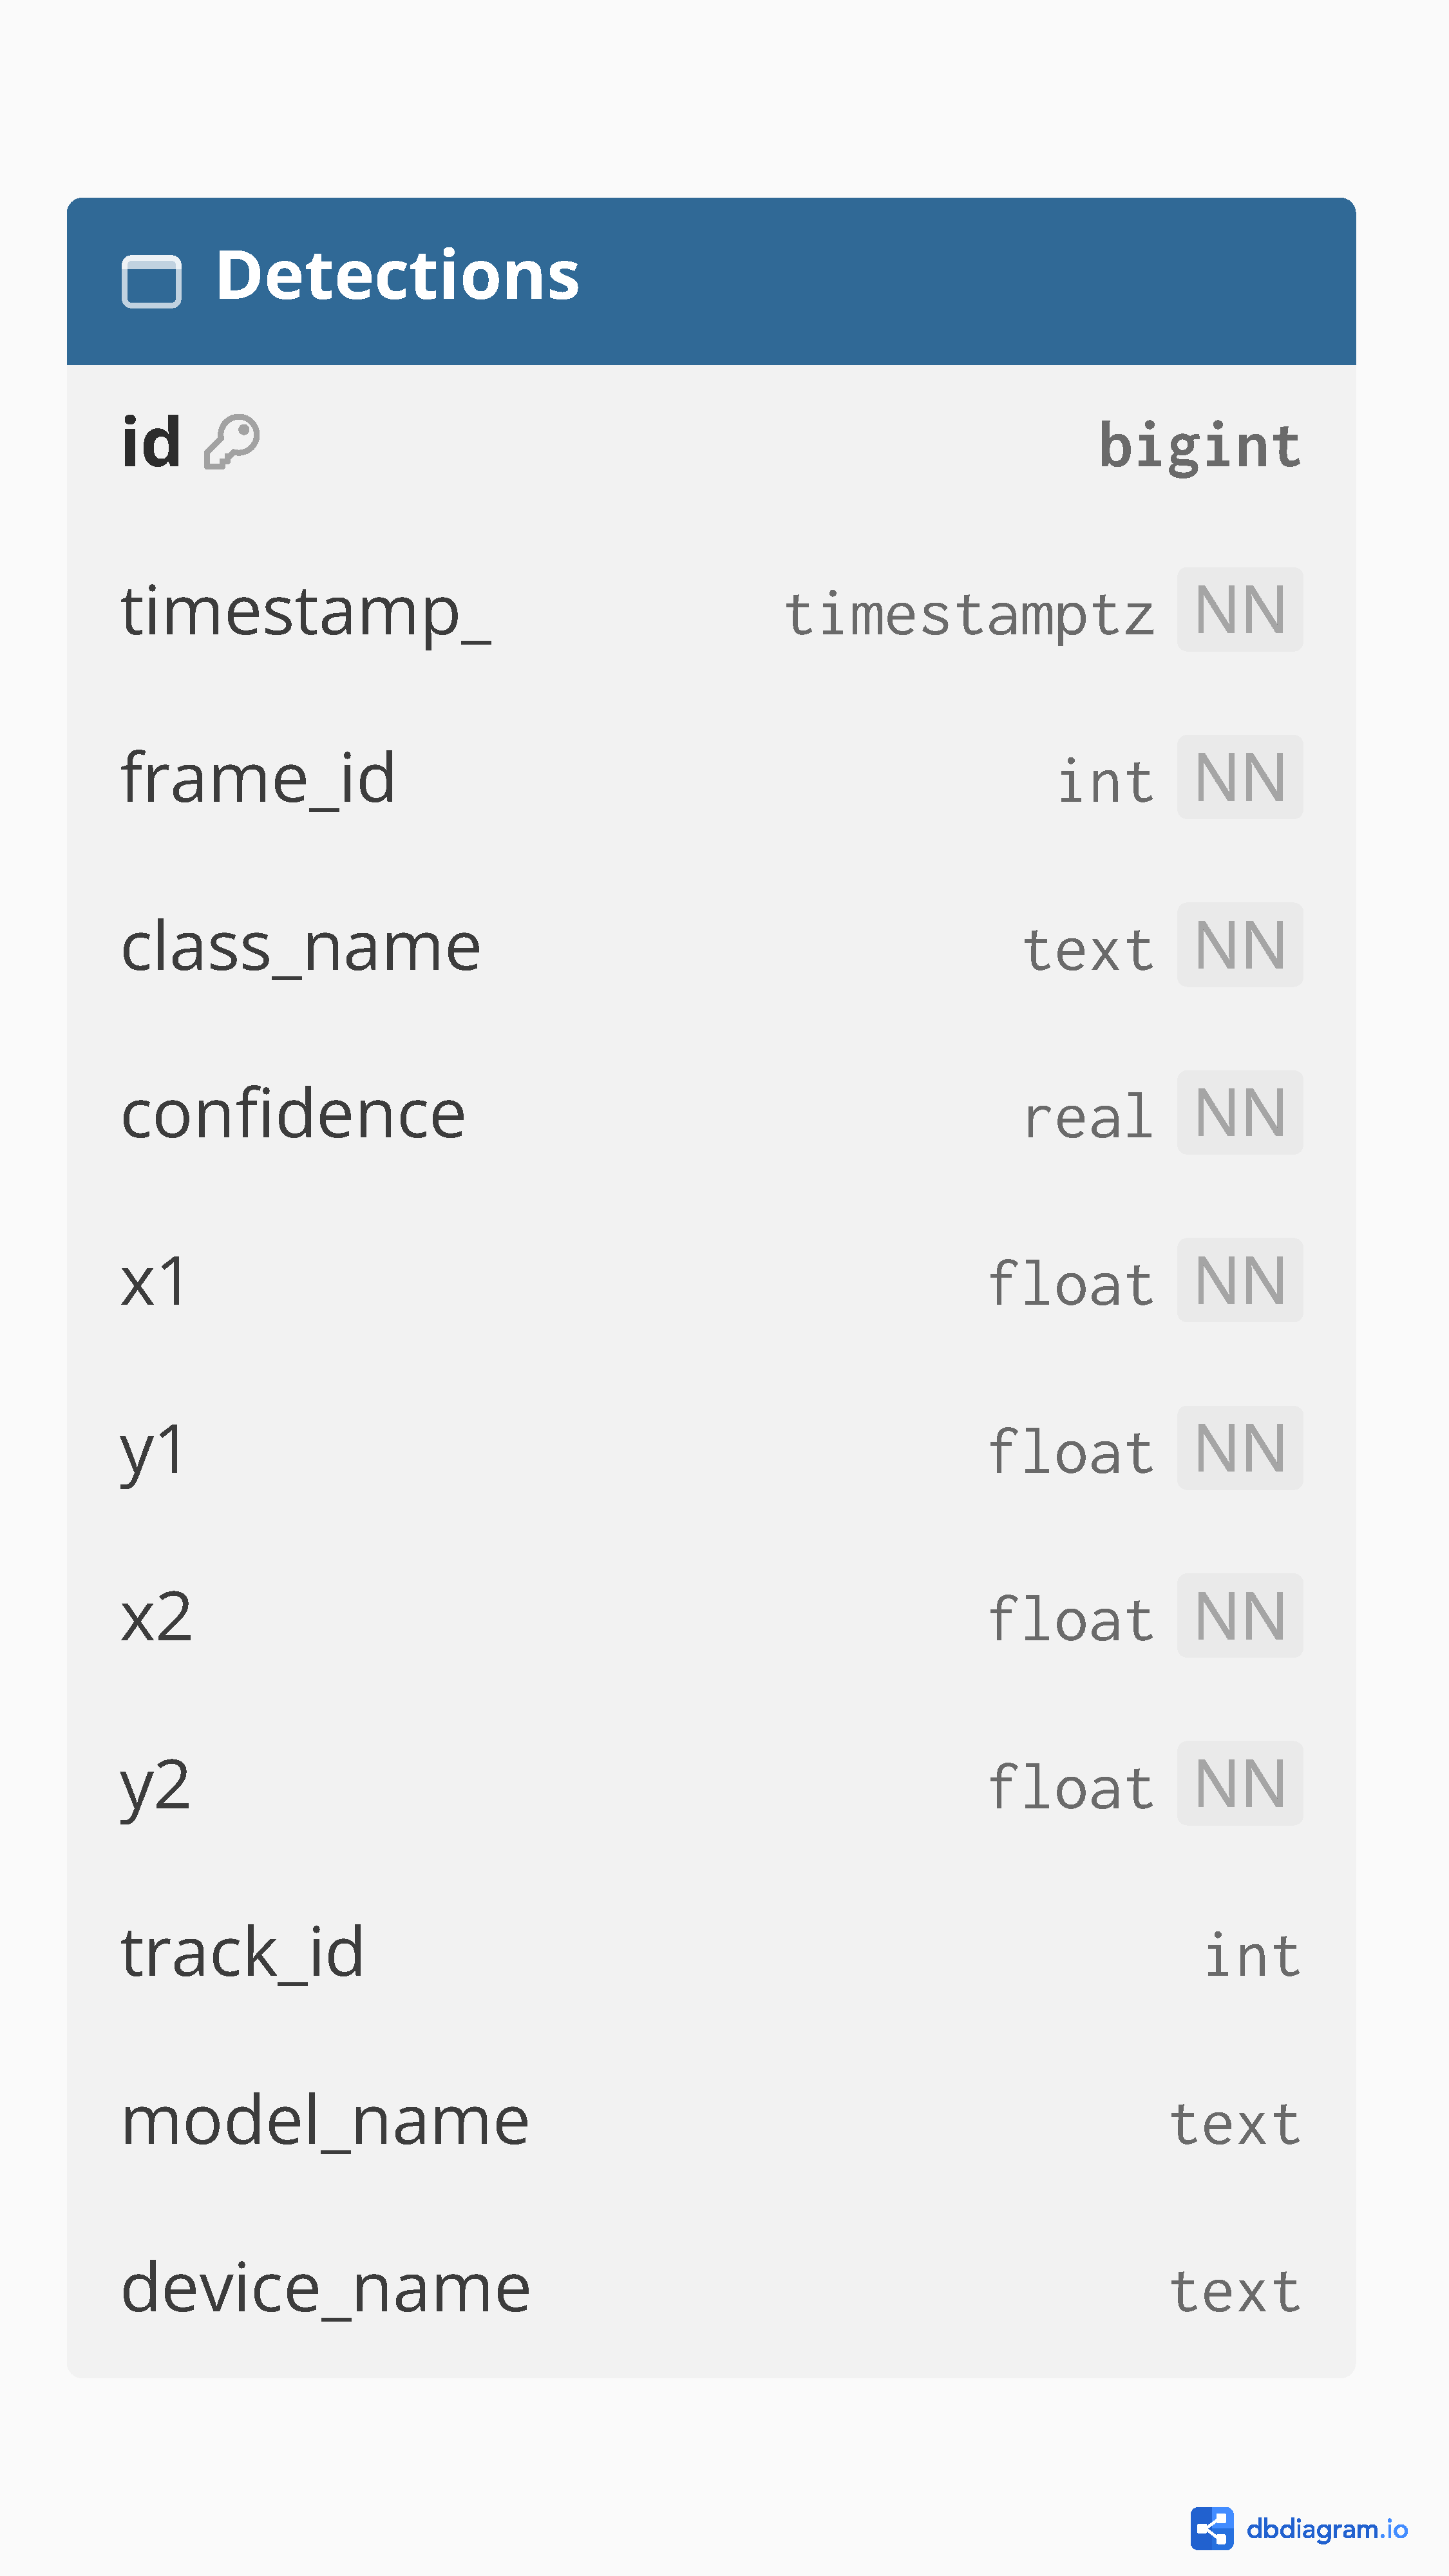
\includegraphics[
        page=1,
        trim={2cm 5cm 2cm 5cm},
        clip,
        width=0.35\textwidth
    ]{images/DB_diagram.pdf}
    \caption{ER diagram databázového modelu.}
    \label{fig:erd}
\end{figure}

\paragraph{Popis atributů tabulky \textit{detections}:}
\begin{itemize}
    \item \textbf{id (BIGSERIAL)} – Primární klíč tabulky. Automaticky generovaná unikátní hodnota sloužící k~jednoznačné identifikaci každé detekce. Typ \textit{BIGSERIAL} byl zvolen s~ohledem na předpokládaný vysoký objem záznamů.
    \item \textbf{timestamp\_ (TIMESTAMPTZ)} – Čas detekce objektu. Datový typ \textit{TIMESTAMPTZ} umožňuje ukládání časové informace včetně časové zóny, což je důležité pro přesnou časovou analýzu dopravních událostí.
    \item \textbf{frame\_id (INTEGER)} – Identifikátor snímku, ve kterém byla detekce provedena. Umožňuje zpětné dohledání konkrétního snímku v~případě analýzy nebo ladění systému.
    \item \textbf{class\_name (TEXT)} – Název detekované třídy objektu (např. \textit{car}, \textit{truck}, \textit{bus}). Tento atribut umožňuje následnou agregaci a statistické vyhodnocení podle typu vozidla.
    \item \textbf{confidence (REAL)} – Pravděpodobnost detekce generovaná neuronovou sítí. Je definováno omezení \texttt{CHECK (confidence >= 0 AND confidence <= 1)}, které zajišťuje validitu ukládaných hodnot.
    \item \textbf{x1, y1, x2, y2 (FLOAT)} – Souřadnice ohraničujícího obdélníku (\textit{bounding box}) detekovaného objektu. Hodnoty představují levý horní a pravý dolní roh objektu v~rámci zpracovávaného obrazu. Integritní omezení \texttt{CHECK (x2 > x1 AND y2 > y1)} zajišťuje geometrickou konzistenci dat.
    \item \textbf{track\_id (INT)} – Identifikátor sledovaného objektu, generovaný sledovacím algoritmem. Umožňuje sledování pohybu konkrétního vozidla napříč více snímky.
    \item \textbf{model\_name (TEXT)} – Označení použitého detekčního modelu (např. \textit{yolov8s}). Sloupec je navržen pro potřeby budoucího porovnávání úspěšnosti různých verzí neuronových sítí nad reálnými daty.
    \item \textbf{device\_name (TEXT)} – Identifikátor konkrétní výpočetní jednotky (edge zařízení) nebo kamery. Zajišťuje připravenost databázového schématu na horizontální škálování systému do více lokalit.
\end{itemize}

\textbf{Indexování:} S~ohledem na charakter dotazů byly vytvořeny indexy nad atributy \textit{timestamp\_}, \textit{class\_name} a \textit{track\_id}. Tyto indexy optimalizují zejména dotazy na poslední detekce, časově omezené statistiky, filtrování podle typu vozidla a analýzu pohybu konkrétního objektu. Použití sestupného indexu nad atributem \textit{timestamp\_} umožňuje efektivní získávání nejnovějších detekcí, což je častý scénář v~reálném provozu systému.

\subsubsection{Analýza a vizualizace dat}
Backendová vrstva zpřístupňuje uložená data prostřednictvím REST API postaveného na moderním frameworku FastAPI. Pro následné numerické transformace a časové agregace záznamů systém využívá knihovny NumPy~\cite{harris_numpy_2020} a Pandas~\cite{mckinney_pandas_2010}. Koncové webové rozhraní s~interaktivními grafy je navrženo s~využitím frameworku Streamlit v~kombinaci s~grafickou knihovnou Plotly~\cite{plotly_docs_2015}, což umožňuje interaktivní zobrazení časových řad, histogramů a agregovaných statistik dopravního provozu.

\subsection{Technologie}
Celkový přehled zvolených technologií pro jednotlivé vrstvy navržené architektury shrnuje tabulka~\ref{tab:tech_stack}.

\begin{table}[H]
    \centering
    \renewcommand{\arraystretch}{1.2}
    \begin{tabular}{|l|l|}
        \hline
        \textbf{Komponenta systému} & \textbf{Zvolená technologie} \\ \hline
        Operační systém (Edge) & Raspberry Pi OS (Debian Linux) \\ \hline
        Programovací jazyk & Python 3.11 \\ \hline
        Zpracování videa & GStreamer \\ \hline
        AI inference a sledování & HailoRT + TAPPAS (YOLO) \\ \hline
        Komunikační protokol & MQTT \\ \hline
        Databázové úložiště & PostgreSQL + Psycopg \\ \hline
        Backend a REST API & FastAPI + Pandas / NumPy \\ \hline
        Vizualizační frontend & Streamlit + Plotly \\ \hline
    \end{tabular}
    \caption{Přehled technologického stacku navrženého systému.}
    \label{tab:tech_stack}
\end{table}

%Výhodou využití frameworku GStreamer je především jeho vysoký výkon a efektivní práce s daty, protože většina jeho pluginů je implementována v jazyce C/C++. Díky tomu může být video stream zpracováván s minimální režijní vrstvou a bez nutnosti přenosu dat mezi interpretem Pythonu a nativním kódem. Jednotlivé prvky pipeline navíc mohou běžet paralelně, což umožňuje efektivní využití systémových prostředků a dosažení vyššího výkonu při zpracování video streamu v reálném čase.

%Pro přenos detekčních událostí mezi edge zařízením a backendovou částí systému je využit protokol MQTT. Tento protokol je vhodný pro lehkou a asynchronní komunikaci v distribuovaných systémech, zejména v prostředí IoT. V navržené architektuře je detekční pipeline zcela oddělena od databázové vrstvy. Edge zařízení publikuje detekční data do MQTT brokeru, zatímco samostatný subscriber modul zajišťuje jejich následné uložení do databáze. Každá detekce je reprezentována strukturou obsahující následující atributy:
%\begin{itemize}
%    \item \textbf{class\_id} – numerický identifikátor třídy,
%    \item \textbf{class\_name} – název detekovaného objektu,
%    \item \textbf{confidence} – pravděpodobnost detekce,
%    \item \textbf{bbox} – souřadnice ohraničujícího obdélníku,
%    \item \textbf{track\_id} – identifikátor sledovaného objektu,
%    \item \textbf{timestamp} – čas detekce.
%\end{itemize}
%Ze získaných detekčních metadat se vytvoří slovník kam se uloží aktuální detekce. Publikace zprávy probíhá pouze v případě, že je seznam detekcí neprázdný a spojení s MQTT brokerem je aktivní. Tím je zajištěno, že do komunikační vrstvy nejsou odesílány redundantní nebo neúplné informace. Databázový modul je implementován jako samostatný MQTT subscriber, který přijímá publikované zprávy a ukládá je do relační databáze PostgreSQL. Tento přístup umožňuje oddělení real-time inference od operací zápisu do databáze, čímž je minimalizováno riziko zpomalení detekční části systému. Identifikátor \textit{track\_id} je označen jako zpracovaný až po úspěšném odeslání zprávy. Tím je zabráněno situaci, kdy by byla detekce považována za odeslanou, aniž by skutečně došlo k jejímu předání komunikační vrstvě.
